\subsection{Task 4: Uber relative excess travel time}
We use only Uber HV0003 trips. The reference is N/N with valid directed OD, pickup and dropoff timestamps, positive timestamp duration, and recorded \texttt{trip\_time} in $(0,24]$ hours. Reference trips from April and May are pooled by ordered OD $\times$ pickup hour $\times$ weekday/weekend (Monday--Friday versus Saturday--Sunday); month is not part of a reference cell. A cell is supported if it contains at least 30 N/N trips. Its median \texttt{trip\_time}/60 is the reference minutes. Each eligible Y/Y trip is matched to its cell; unsupported comparisons have null $E$ and $R$.
For trip $i$, $E_i=T_i-T_{ref,i}$ minutes and $R_i=100E_i/T_{ref,i}$ percent. Negative values are retained. Each trip receives equal weight in all medians, quartiles, and zone means; cells do not receive equal weight. Relative differences are calculated for individual trips before aggregation.
\begin{table}[htbp]\centering\scriptsize\caption{Uber Y/Y reference coverage and trip-weighted excess-time summaries. IQR endpoints are the 25th and 75th percentiles.}\label{tab:t4summary}\begin{tabular}{lrrrrrr}\hline Month & Eligible Y/Y & Supported & Coverage \% & Median $E$ & $E$ IQR & Median $R$ \% \\ \hline
2026-04 & 255,383 & 121,673 & 47.6 & 4.53 & [0.25, 10.01] & 25.8 \\
2026-05 & 220,904 & 110,559 & 50.0 & 4.98 & [0.71, 10.48] & 29.4 \\
\hline\end{tabular}\end{table}
For Uber, 29,927,521 N/N and 476,289 Y/Y completed OD trips pass the timestamp and zone checks; 75 N/N and 2 Y/Y records are then excluded for invalid recorded trip time. No completed Uber trip has a missing or invalid OD zone in these files.
The supported reference contains 211,171 cells, covering 22,768,936 of 29,927,446 eligible N/N records. Among shared trips without a supported comparison, 21,055 have no N/N cell at all and 223,000 have a cell with fewer than 30 N/N trips. April's relative-excess IQR is [1.5, 55.0]\%; May's is [4.5, 58.9]\%. The hourly and zone CSV supplements give both full IQRs and coverage denominators.
\begin{figure}[htbp]\centering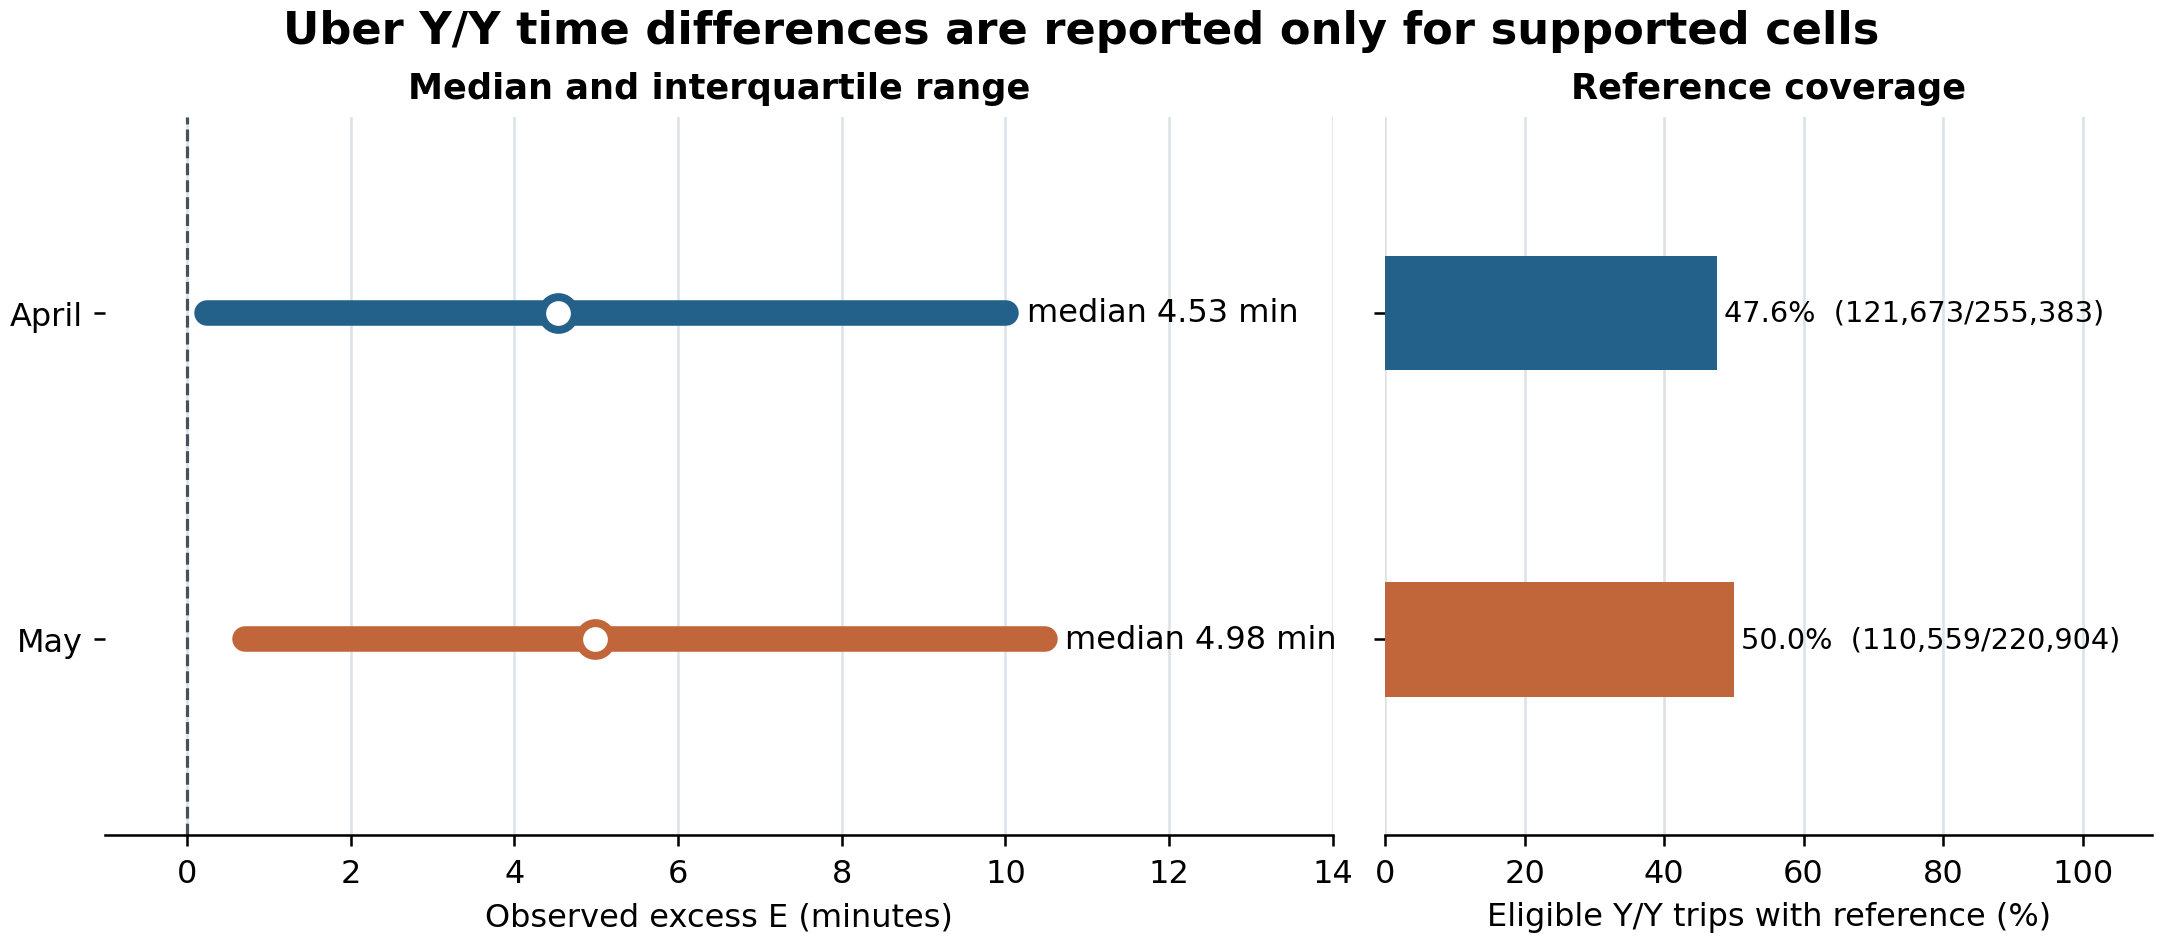
\includegraphics[width=.48\textwidth]{04_Results/Task_4/figures/monthly_coverage_excess.png}\hfill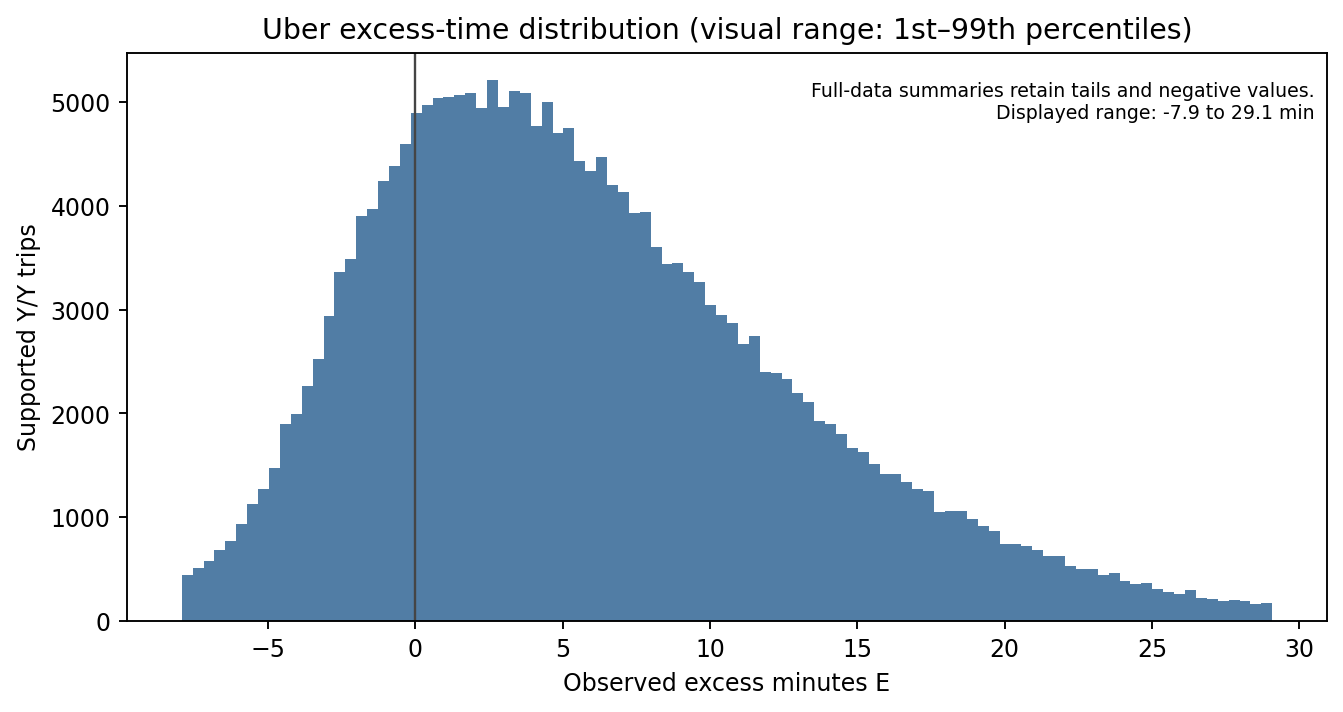
\includegraphics[width=.48\textwidth]{04_Results/Task_4/figures/excess_distribution.png}\caption{Month coverage and excess-time distribution. Histogram tails are trimmed for display only; statistical summaries use all supported trips.}\label{fig:t4summary}\end{figure}
\begin{figure}[htbp]\centering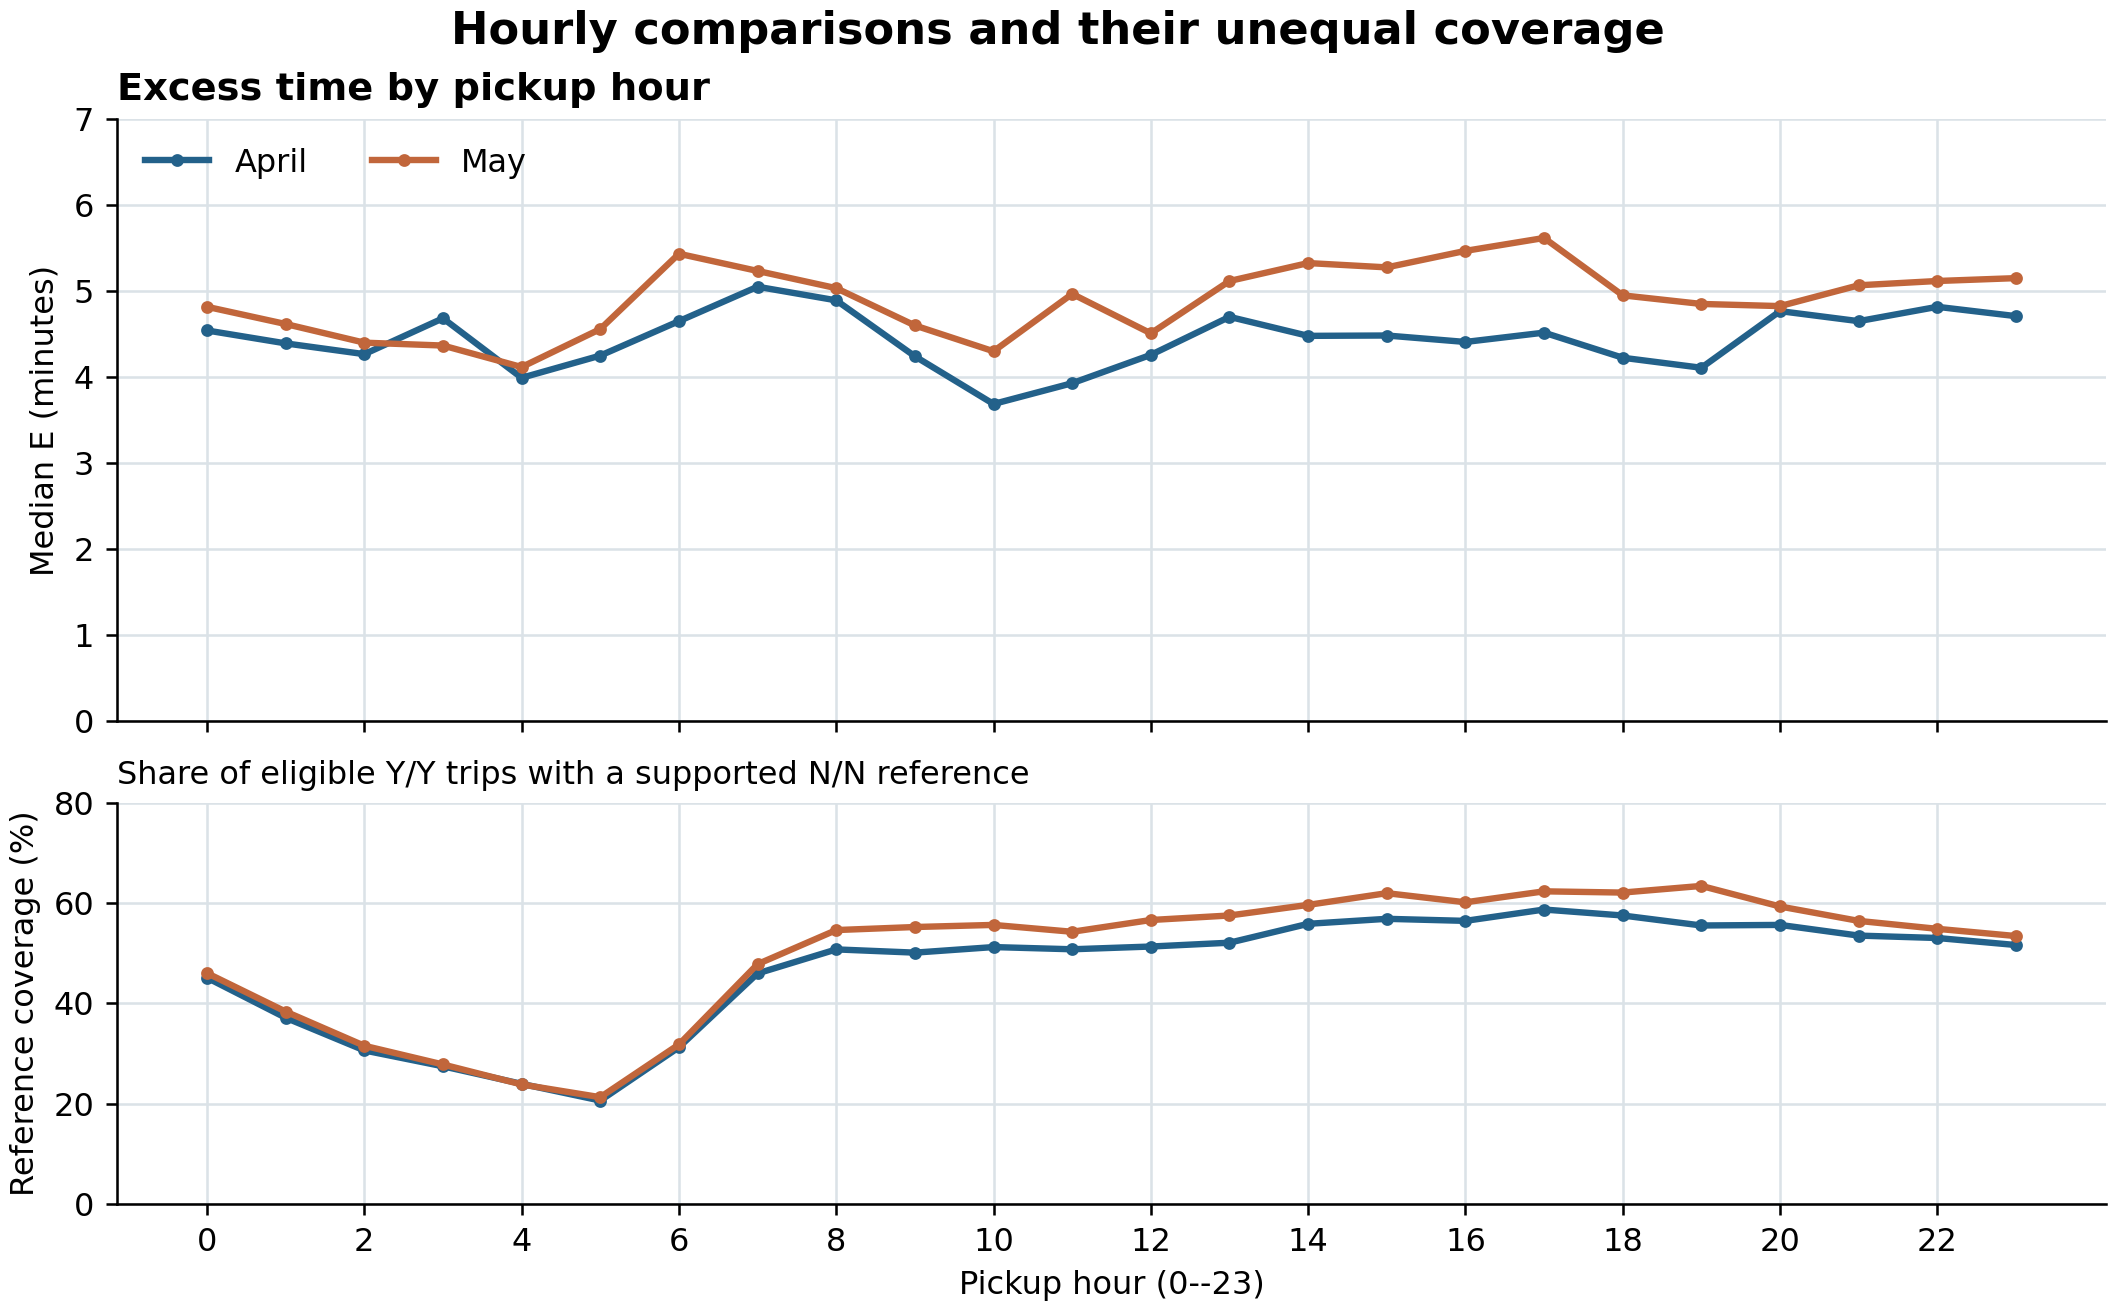
\includegraphics[width=.48\textwidth]{04_Results/Task_4/figures/hourly_excess_minutes.png}\hfill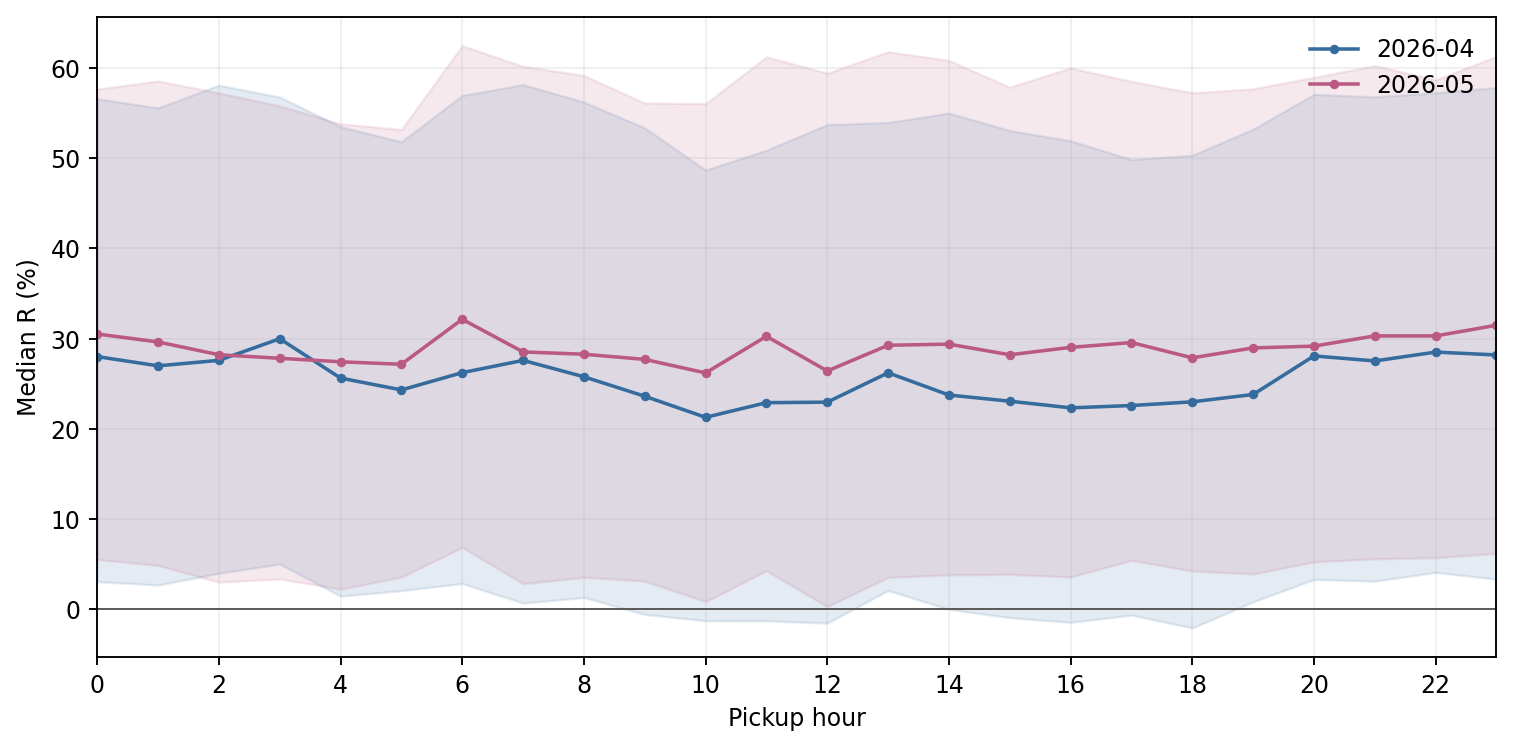
\includegraphics[width=.48\textwidth]{04_Results/Task_4/figures/hourly_relative_percent.png}\caption{Trip-weighted hourly medians and interquartile bands by pickup month.}\label{fig:t4hour}\end{figure}
\begin{figure}[htbp]\centering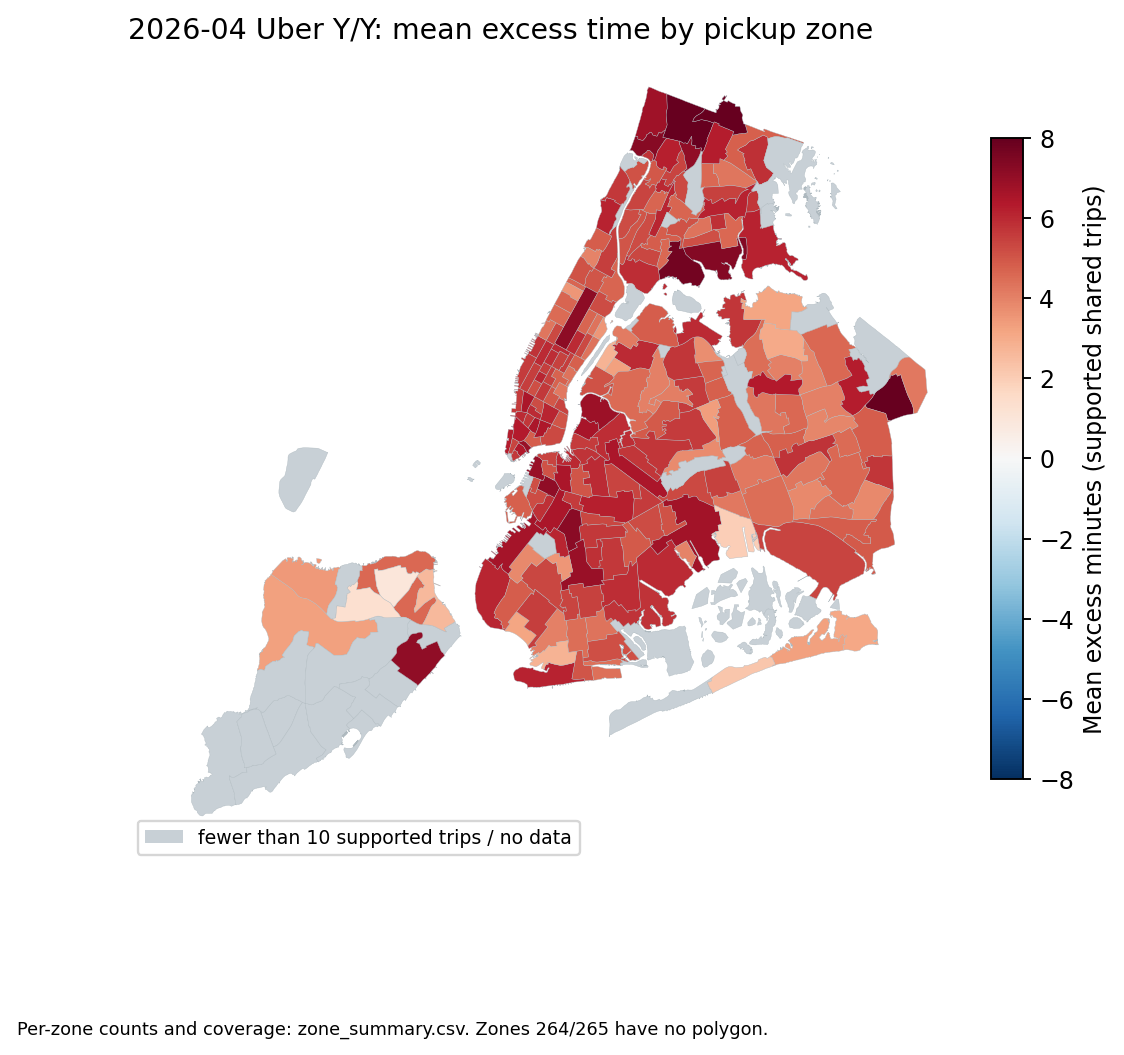
\includegraphics[width=.47\textwidth]{04_Results/Task_4/figures/mean_excess_zone_2026-04.png}\hfill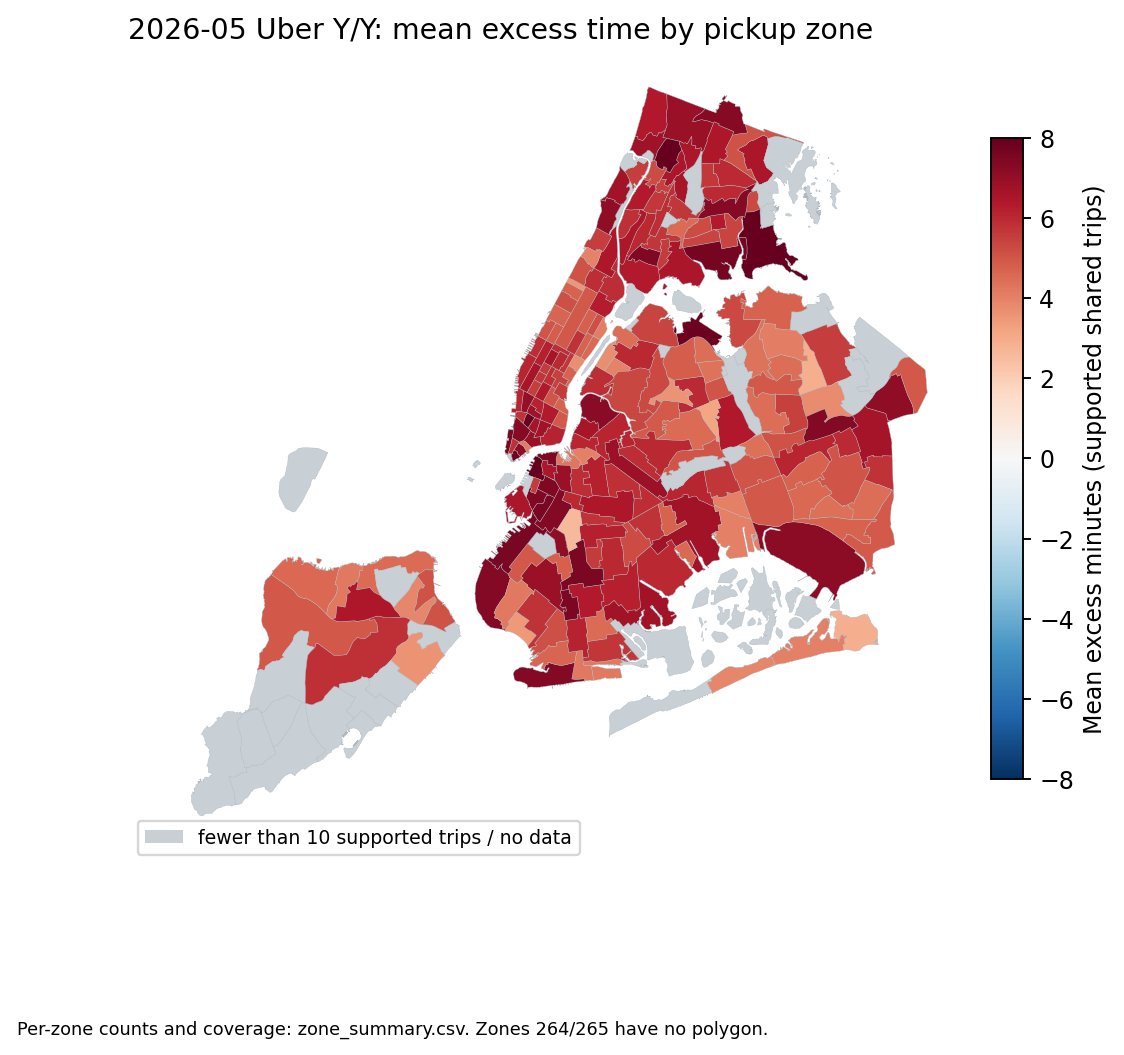
\includegraphics[width=.47\textwidth]{04_Results/Task_4/figures/mean_excess_zone_2026-05.png}\caption{Mean non-null excess minutes by pickup zone, displayed only with at least 10 supported shared trips per month. Both maps share one color scale.}\label{fig:t4zone}\end{figure}
Between-zone Y/Y trips have median $E=4.86$ min and median $R=27.4\%$ among 226,297 supported trips; reference coverage is 48.1\%.
Within-zone Y/Y trips have median $E=2.00$ min and median $R=31.4\%$ among 5,935 supported trips; reference coverage is 98.7\%.
In 2026-04, the lowest hourly median $E$ was 3.69 min at 10:00 and the highest was 5.05 min at 07:00; hourly reference coverage varies, so these are comparisons among supported trips only.
In 2026-05, the lowest hourly median $E$ was 4.12 min at 04:00 and the highest was 5.62 min at 17:00; hourly reference coverage varies, so these are comparisons among supported trips only.
Among 165 2026-04 pickup zones with at least 100 supported shared trips, the lowest mean $E$ was Howard Beach (1.98 min) and the highest was Woodlawn/Wakefield (8.30 min). The map includes zones with at least 10 supported trips and clips its color at 8 min for readability; underlying CSV means are untrimmed.
Among 162 2026-05 pickup zones with at least 100 supported shared trips, the lowest mean $E$ was Rego Park (3.17 min) and the highest was Schuylerville/Edgewater Park (8.56 min). The map includes zones with at least 10 supported trips and clips its color at 8 min for readability; underlying CSV means are untrimmed.
This is an observed comparison, not a causal pooling effect. Trips sharing a TLC zone pair can have different exact endpoints; traffic varies by date even within the same hour/day-type cell; routes and passenger selection differ. The flags do not verify a specific sharing partner or overlap time. Reference coverage also varies by location, so mapped averages reflect a selected subset. The N/N median is an observed reference, not an optimal or congestion-free travel time. The zone coverage map and CSV make that selection visible.
